\newtoggle{withbonus} \toggletrue{withbonus} % set true to show bonus points in grade table

% setting underlying course name (Grundlagenfach Mathematik, §-Unterricht, \ldots)
\newcommand{\mycourse}{Grundlagenfach Informatik}
% name of the class
\newcommand{\myclass}{2. Klassen}
% set date
\newcommand{\mydate}{09. November 2023}

\title{\textbf{Aufgabensammlung}}
\author{Autoren: Patrick Hnilicka, Michael Anderegg, Cyril Wendl, Thomas Graf\\
\mycourse, \myclass}
\date{\mydate}
\maketitle
\thispagestyle{headandfoot}		

\begin{center}
	\fbox{\parbox{140mm}{\centering
			\begin{itemize}
				\item Dauer der Prüfung: $45$ Minuten.
				%\item \textbf{Zeige in jeder Aufgabe unbedingt Deine Schritte!}
				\item Erlaubte Hilfsmittel:
				\begin{itemize}
				    \item Schreibzeug
				    %\item Taschenrechner
				\end{itemize}
	\end{itemize}}}
\end{center}
\vspace{10mm}

\begin{center}
	Vorname: \rule{45mm}{0.8pt}\qquad Nachname: \rule{45mm}{0.8pt}
\end{center}
\vspace{20mm}

\begin{center}
	\iftoggle{withbonus} {
		\combinedgradetable[h][questions]
	} {
		\gradetable[h][questions]
	}
\end{center}
\vspace{15mm}
\begin{center}
	Note: 
	\vspace{10mm}
	
	\rule{8mm}{1.2pt}
\end{center}
%\thispagestyle{empty}
\clearpage

\begin{questions}
\section{Zahlensysteme}
\question[2]{\textbf{Umrechnen in das 5-adische Zahlensystem}}

Wie lautet die kürzeste Darstellung der natürlichen Zahl 72 im 5-adischen System (Basis 5)?
\begin{solution}
Wir berechnen einige Potenzen der Basis 5:
\begin{align*}
    5^3 = 125, \quad 5^2 = 25, \quad 5^1 = 5, \quad 5^0 = 1
\end{align*}
und somit (Ausschöpfen von 72 durch stets möglichst viele der grösstmöglichen Potenzen von 5):
\begin{align*}
    72 = 2\cdot 5^2 + 4\cdot 5^1 + 2\cdot 5^0 = 242_5.
\end{align*}
\end{solution}
\droptotalpoints

\question{\textbf{Zahlensysteme umrechnen}}
\begin{parts}
    \part[1] Wie lautet die kürzeste Darstellung der natürlichen Zahl 53 im 3-adische Zahlensystem (Basis 3)?
    \begin{solution}
    Wir berechnen einige Potenzen der Basis 3:
    \begin{align*}
        3^3 = 27, \quad 3^2 = 9, \quad 3^1 = 3, \quad 3^0 = 1
    \end{align*}
    und somit (Ausschöpfen von 53 durch stets möglichst viele der grösstmöglichen Potenzen von 3):
    \begin{align*}
        53 = 1\cdot 3^3 + 2\cdot 3^2 + 2\cdot 3^1 + 2\cdot3^0 = 1222_3.
    \end{align*}
    \end{solution}
    \part[2] Begründen Sie, weshalb die Ansammlung
    \begin{center}
        \coin{1}\coin{7}\coin{40}\coin{49}
    \end{center}
    von Münzen keine gültige \textit{Münzendarstellung} im 7-adischen Zahlensystem ist.
    \begin{solution}
        Die Zahl 40 ist keine gültige Basisgrösse des 7-adischen Zahlensystems ($7^2 = 49, \quad 7^1 = 7, \quad 7^0 = 1$).
    \end{solution}
    \part[1] Stellen Sie die beiden natürlichen Zahlen 7 und 11 binär dar. Führen Sie danach die binäre schriftliche Addition dieser beiden gefundenen Darstellungen durch. Zeigen Sie Ihre Schritte.
    \begin{solution}
    Die binäre Darstellung von 7 ist $111_2$ und die von 11 ist $1011_2$. Ihre (binäre) schriftliche Addition lautet:
        \begin{center}
            \begin{tabular}{cccccc}
                    & 0 & 0 & 1 & 1 & 1 \\
                +   & 0 & 1 & 0 & 1 & 1 \\
                \hline
                    & 1 & 0 & 0 & 1 & 0
            \end{tabular}
        \end{center}
    \end{solution}
\end{parts}
\droptotalpoints


\section{Graphen}

\question[3]{\textbf{Bäume}\\
Bestimmen Sie, welche der folgenden Graphen auch Bäume sind:}\\
\begin{oneparchoices}
	\choice
	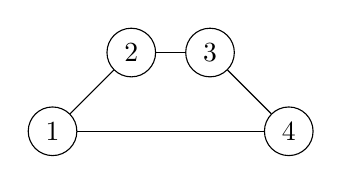
\begin{tikzpicture}
	  \node[circle, draw] (1) at (0,0) {1};
	  \node[circle, draw] (2) at (1,1) {2};
	  \node[circle, draw] (3) at (2,1) {3};
	  \node[circle, draw] (4) at (3,0) {4};
	  
	  \draw (1) -- (2);
	  \draw (2) -- (3);
	  \draw (3) -- (4);
	  \draw (4) -- (1);
	\end{tikzpicture}	
	\choice
	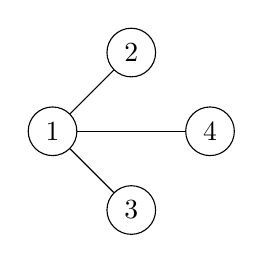
\begin{tikzpicture}
	  \node[circle, draw] (1) at (0,0) {1};
	  \node[circle, draw] (2) at (1,1) {2};
	  \node[circle, draw] (3) at (1,-1) {3};
	  \node[circle, draw] (4) at (2,0) {4};
	  
	  \draw (1) -- (2);
	  \draw (1) -- (3);
	  \draw (1) -- (4);
	\end{tikzpicture}
	\correctchoice
		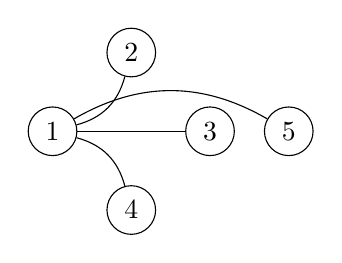
\begin{tikzpicture}
		  \node[circle, draw] (1) at (0,0) {1};
		  \node[circle, draw] (2) at (1,1) {2};
		  \node[circle, draw] (3) at (2,0) {3};
		  \node[circle, draw] (4) at (1,-1) {4};
		  \node[circle, draw] (5) at (3,0) {5};
		  
		  \draw (1) to [bend right=30] (2);
		  \draw (1) -- (3);
		  \draw (1) to [bend left=30] (4);
		  \draw (1) to [bend left=30] (5);
		\end{tikzpicture}
	\choice
	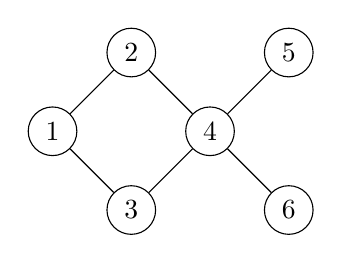
\begin{tikzpicture}
	  \node[circle, draw] (1) at (0,0) {1};
	  \node[circle, draw] (2) at (1,1) {2};
	  \node[circle, draw] (3) at (1,-1) {3};
	  \node[circle, draw] (4) at (2,0) {4};
	  \node[circle, draw] (5) at (3,1) {5};
	  \node[circle, draw] (6) at (3,-1) {6};
	  
	  \draw (1) -- (2);
	  \draw (1) -- (3);
	  \draw (3) -- (4);
	  \draw (4) -- (2);
	  \draw (4) -- (5);
	  \draw (4) -- (6);
	\end{tikzpicture}
	\correctchoice
		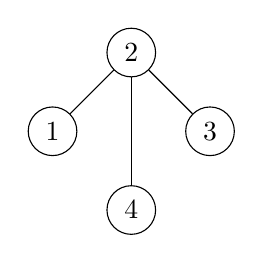
\begin{tikzpicture}
		  \node[circle, draw] (1) at (0,0) {1};
		  \node[circle, draw] (2) at (1,1) {2};
		  \node[circle, draw] (3) at (2,0) {3};
		  \node[circle, draw] (4) at (1,-1) {4};
		  
		  \draw (1) -- (2);
		  \draw (2) -- (3);
		  \draw (2) -- (4);
		\end{tikzpicture}
	\choice
	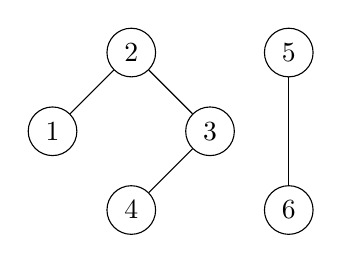
\begin{tikzpicture}
	  \node[circle, draw] (1) at (0,0) {1};
	  \node[circle, draw] (2) at (1,1) {2};
	  \node[circle, draw] (3) at (2,0) {3};
	  \node[circle, draw] (4) at (1,-1) {4};
	  \node[circle, draw] (5) at (3,1) {5};
	  \node[circle, draw] (6) at (3,-1) {6};
	  
	  \draw (1) -- (2);
	  \draw (2) -- (3);
	  \draw (3) -- (4);
	  \draw (5) -- (6);
	\end{tikzpicture}
	\\
	\correctchoice
	\begin{tikzpicture}
	% 	\draw [help lines] (0,0) grid (10,10);
	\scriptsize
     	\tikzstyle{c} = [draw, shape=circle, anchor=center, minimum width=.7cm]
    	\node[c](II){II};
    	\node[c, right=1cm of II](V){V} edge (II);
    	\node[c, below=1cm of V](IV){IV} edge (V);
    	\node[c, left=1cm of IV](III){III} edge (II);
    	\node[c, left=1cm of II](VI){VI};
    	\node[c, below=1cm of VI](I){I} edge (VI) edge (III);
    	\node[c, left=1cm of VI](VII){VII} edge (VI);
	\end{tikzpicture}
\end{oneparchoices}
\droptotalpoints
\question[3]{\textbf{Bäume}\\
Bestimmen Sie, welche der folgenden Graphen auch Bäume sind:}
\begin{oneparchoices}
	\correctchoice
		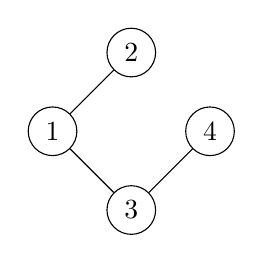
\begin{tikzpicture}
		  \node[circle, draw] (1) at (0,0) {1};
		  \node[circle, draw] (2) at (1,1) {2};
		  \node[circle, draw] (3) at (1,-1) {3};
		  \node[circle, draw] (4) at (2,0) {4};
		  
		  \draw (1) -- (2);
		  \draw (1) -- (3);
		  \draw (3) -- (4);
		\end{tikzpicture}
		\choice 
		\begin{tikzpicture}
		% 	\draw [help lines] (0,0) grid (10,10);
		\scriptsize
		      	\tikzstyle{c} = [draw, shape=circle, anchor=center, minimum width=.7cm]
		     	\node[c](II){II};
		     	\node[c, right=1cm of II](V){V} edge (II);
		     	\node[c, below=1cm of V](IV){IV} edge (V);
		     	\node[c, left=1cm of IV](III){III} edge (II);
		     	\node[c, left=1cm of II](VI){VI};
		     	\node[c, below=1cm of VI](I){I} edge (VI);
		     	\node[c, left=1cm of VI](VII){VII} edge (VI);
		\end{tikzpicture}
	\choice
	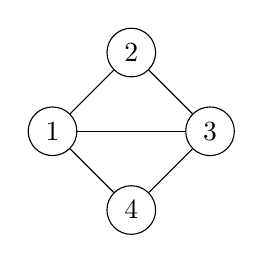
\begin{tikzpicture}
	  \node[circle, draw] (1) at (0,0) {1};
	  \node[circle, draw] (2) at (1,1) {2};
	  \node[circle, draw] (3) at (2,0) {3};
	  \node[circle, draw] (4) at (1,-1) {4};
	  
	  \draw (1) -- (2);
	  \draw (2) -- (3);
	  \draw (3) -- (4);
	  \draw (4) -- (1);
	  \draw (1) -- (3);
	\end{tikzpicture}\\
	\correctchoice 
	    \begin{tikzpicture}
	    % 	\draw [help lines] (0,0) grid (10,10);
	    \scriptsize
	     	\tikzstyle{c} = [draw, shape=circle, anchor=center, minimum width=.7cm]
	    	\node[c](II){II};
	    	\node[c, right=1cm of II](V){V} edge (II);
	    	\node[c, below=1cm of V](IV){IV} edge (V);
	    	\node[c, left=1cm of IV](III){III} edge (II);
	    	\node[c, left=1cm of II](VI){VI} edge (II);
	    	\node[c, below=1cm of VI](I){I} edge (VI);
	    	\node[c, left=1cm of VI](VII){VII} edge (VI);
	   \end{tikzpicture}
	\choice
	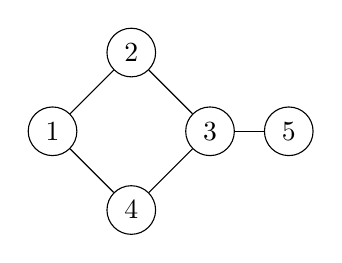
\begin{tikzpicture}
	  \node[circle, draw] (1) at (0,0) {1};
	  \node[circle, draw] (2) at (1,1) {2};
	  \node[circle, draw] (3) at (2,0) {3};
	  \node[circle, draw] (4) at (1,-1) {4};
	  \node[circle, draw] (5) at (3,0) {5};
	  
	  \draw (1) -- (2);
	  \draw (2) -- (3);
	  \draw (4) -- (3);
	  \draw (1) -- (4);
	  \draw (3) -- (5);
	\end{tikzpicture}
	\choice
	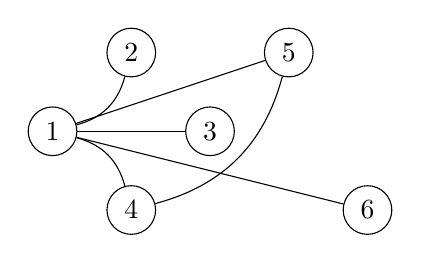
\begin{tikzpicture}
	  \node[circle, draw] (1) at (0,0) {1};
	  \node[circle, draw] (2) at (1,1) {2};
	  \node[circle, draw] (3) at (2,0) {3};
	  \node[circle, draw] (4) at (1,-1) {4};
	  \node[circle, draw] (5) at (3,1) {5};
	  \node[circle, draw] (6) at (4,-1) {6};
	  
	  \draw (1) to [bend right=30] (2);
	  \draw (1) -- (3);
	  \draw (1) to [bend left=30] (4);
	  \draw (4) to [bend right=30]  (5);
	  \draw (1) to (5);
	  \draw (1) to (6);
	\end{tikzpicture}
	\choice 
	 \begin{tikzpicture}
	 % 	\draw [help lines] (0,0) grid (10,10);
	 \scriptsize
	  	\tikzstyle{c} = [draw, shape=circle, anchor=center, minimum width=.7cm]
	 	\node[c](II){II};
	 	\node[c, right=1cm of II](V){V} edge (II);
	 	\node[c, below=1cm of II](III){III} edge (II);
	 	\node[c, left=1cm of II](VI){VI} edge (II) edge (III);
	 	\node[c, below=1cm of VI](I){VI} edge (VI);
	 \end{tikzpicture}
	 \correctchoice 
	  \begin{tikzpicture}
	  % 	\draw [help lines] (0,0) grid (10,10);
	  \scriptsize
	   	\tikzstyle{c} = [draw, shape=circle, anchor=center, minimum width=.7cm]
	  	\node[c](II){II};
	  	\node[c, right=1cm of II](V){V} edge (II);
	  	\node[c, below=1cm of V](IV){IV} edge (V);
	  	\node[c, left=1cm of IV](III){III} edge (IV);
	  	\node[c, left=1cm of II](VI){VI} edge (II);
	  \end{tikzpicture}
\end{oneparchoices}
\droptotalpoints

\newcommand{\tikzWinti}{
\begin{tikzpicture}[inner sep=2pt]
% 	\draw [help lines] (0,0) grid (10,10);
 	\tikzstyle{c} = [draw, shape=circle]
	\node[c](1){1};
	\node[c, right=1cm of 1](2){2} edge (1);
	\node[c, below=1cm of 2](3){3} edge (2);
	\node[c, left=1cm of 3](7){7} edge (3) edge (1) edge (2);
	\node[c, left=1cm of 1](4){4} edge (1);
	\node[c, above=1cm of 4](6){6} edge (1) edge (4);
	\node[c, right=1cm of 6](5){5} edge (6) edge (1);
\end{tikzpicture}
}
\newcommand{\tikzBern}{
\begin{tikzpicture}
% 	\draw [help lines] (0,0) grid (10,10);
\scriptsize
 	\tikzstyle{c} = [draw, shape=circle, anchor=center, minimum width=.7cm]
	\node[c](II){II};
	\node[c, right=1cm of II](V){V} edge (II);
	\node[c, below=1cm of V](IV){IV} edge (V);
	\node[c, left=1cm of IV](III){III} edge (IV) edge (II);
	\node[c](I) at ($(II)!0.5!(IV)$) {I} edge (II) edge (V) edge (IV) edge (III);
	\node[c, left=1cm of I](VI){VI} edge (II) edge (III);
\end{tikzpicture}
}

\newcommand{\tikzThurgau}{
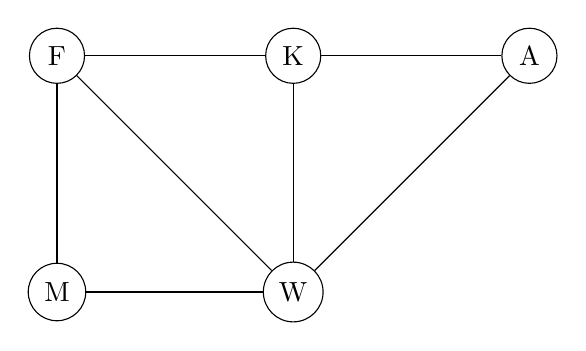
\begin{tikzpicture}[node distance=2cm]
	\tikzstyle{c} = [draw, shape=circle, anchor=center, minimum width=.7cm]
  % Bezirke
  \node[c] (f) at (0,3) {F};
  \node[c] (m) at (0,0) {M};
  \node[c] (k) at (3,3) {K};
  \node[c] (w) at (3,0) {W}; 
  \node[c] (a) at (6,3) {A};

  % Verbindungen
  \draw (f) -- (k);
  \draw (f) -- (w);
  \draw (f) -- (m);
  \draw (m) -- (w);
  \draw (k) -- (w);
  \draw (k) -- (a);
  \draw (w) -- (a);
\end{tikzpicture}

}
\newcommand{\matrixBern}{
\begin{tabular}{c|c|c|c|c|c|c}
&\textbf{I}&\textbf{II}&\textbf{III}&\textbf{IV}&\textbf{V}&\textbf{VI}\\\midrule
\textbf{I}&0&1&1&1&1&0\\
\textbf{II}&1&0&1&0&1&1\\
\textbf{III}&1&1&0&1&0&1\\
\textbf{IV}&1&0&1&0&1&0\\
\textbf{V}&1&1&0&1&0&0\\
\textbf{VI}&0&1&1&0&0&0\\
\end{tabular}
}

\newcommand{\matrixWinti}{
\begin{tabular}{c|c|c|c|c|c|c|c}
&\textbf{1}&\textbf{2}&\textbf{3}&\textbf{4}&\textbf{5}&\textbf{6}&\textbf{7}\\\midrule
\textbf{1}&0&1&0&1&1&1&1\\
\textbf{2}&1&0&1&0&0&0&1\\
\textbf{3}&0&1&0&0&0&0&1\\
\textbf{4}&1&0&0&0&0&1&0\\
\textbf{5}&1&0&0&0&0&1&0\\
\textbf{6}&1&0&0&1&1&0&0\\
\textbf{7}&1&1&1&0&0&0&0\\
\end{tabular}
}

\newcommand{\matrixThurgau}{
\begin{tabular}{c|c|c|c|c|c}
&\textbf{F}&\textbf{M}&\textbf{K}&\textbf{W}&\textbf{A}\\\midrule
\textbf{F}&0&1&1&1&0\\
\textbf{M}&1&0&0&1&0\\
\textbf{K}&1&0&0&1&1\\
\textbf{W}&1&1&1&0&1\\
\textbf{A}&0&0&1&1&0\\
\end{tabular}
}

\foreach \ort/\einheitPl/\bspnummer/\bspname/\fgwdth/\tikzStadt/\solB/\solC/\solD in {
Winterthur/Stadtkreise/6/Wülflingen/.75/\tikzWinti/{Nein, es gibt keinen Euler'schen Weg, da mehr als zwei Knoten einen ungeraden Grad haben. Es gibt viele Hamilton'sche Wege, beispielsweise 7-3-2-1-4-6-5-1, aber keinen Hamilton'schen Kreis.}/{Der Grad des Grafen ist 5 (von Knoten 1).}/\matrixWinti, 
Bern/Stadtteile/I/Innere Stadt/.95/\tikzBern/{Ja, der Graph enthält den Euler'schen Weg IV-I-V-IV-III-I-II-III-VI-II-V. Der Graph enthält viele Hamilton'sche Kreise, beispielsweise VI-II-V-I-IV-III-VI.}/{Der Grad des Grafen ist 4 (von Knoten I).}/\matrixBern,
Thurgau/Bezirke/M/Münchenwilen/.95/\tikzThurgau/{Ja, der Graph enthält Euler'sche Wege, beispielsweise F-M-W-F-K-W-A-K. Der Graph enthält viele Hamilton'sche Kreise, beispielsweise W-M-F-K-A-W.}/{Der Grad des Grafen ist 4 (von Knoten W).}/\matrixThurgau
%
}{
\question{\textbf{\einheitPl{} von \ort}}\\
Sie betrachten folgende Karte der \einheitPl{} von \ort.\\
\begin{figure}[H]
	\centering
	\includegraphics[width=\fgwdth\textwidth]{GrundlagenInfo/ExamQuestions/Figures/Karte \ort\einheitPl}
\end{figure}
\begin{parts}
\part[2] Zeichnen Sie die Karte als Graphen, wobei jeder der \einheitPl{} ein Knoten sein soll und zwischen zwei Knoten jeweils eine Kante besteht, sofern zwei \einheitPl{} von \ort{} aneinandergrenzen. Als Namen der Knoten können Sie eine Abkürzung wählen (also z.B. ``\bspnummer'' für \bspname).
\begin{solution}
\begin{figure}[H]
\centering
\tikzStadt
\end{figure}
\end{solution}
\part[2] Gibt es  auf diesem Graphen Euler'sche Wege? Gibt es Hamilton'sche Kreise? Falls ja, notieren Sie die Knotenfolge für einen Euler'schen Weg, beziehungsweise einen Hamilton'schen Kreis.
\begin{solution}
\solB
\end{solution}
\part[1] Was ist der Grad dieses Graphen?
\begin{solution}
\solC
\end{solution}
\part[2] Zeichnen Sie die Nachbarschaftsmatrix des Graphen.
\begin{solution}
\begin{table}[H]
\centering
\solD
\end{table}
\end{solution}
\end{parts}
\droptotalpoints
}

\section{Geheimschriften}
\question[1]{Was berechnet die Friedmann'sche Charakteristik? Kreuzen Sie die richtige Antwort an:}\\
\begin{choices}
 \correctchoice Die Friedmann'sche Charakteristik $FC$ eines Texts $T$ ($FC_T$) berechnet die Schlüssellänge durch als die Summe der Abweichungen (im Quadrat) der Häufigkeit aller Zahlen von der erwarteten Häufigkeit (1/26). Für deutsche Text ist $FC_T\sim 0.0388$.
 \choice Die Friedmann'sche Charakteristik $FC$ eines Texts $T$ ($FC_T$) berechnet die Schlüssellänge, indem die häufigsten Bi- oder Trigramme in einem Text gesucht werden und deren Abstände berechnet und in Primfaktoren zerlegt werden. Die am häufigsten vorkommenden Primfaktoren bestimmen die Schlüssellänge.
 \choice Die Friedmann'sche Charakteristik erlaubt es uns, mit Vigenère verschlüsselte Geheimtexte zurück in den Klartext umzuwandeln, indem eine Häufigkeitsanalyse im ursprünglichen Text durchgeführt wird. Der am häufigsten vorkommende Buchstabe im Geheimtext entspricht bei genug langer Textlänge erwartungsgemäss dem häufigsten Buchstaben in der jeweiligen Sprache des Klartext.
\end{choices}
\droptotalpoints

\section{Kompression}
\question
        Gesucht sind zwei unterschiedliche binäre Kodierungen für die Buchstaben H, E, L, O.
        \begin{parts}
            \part[2] Geben Sie in der Tabelle eine Kodierung an, die \textbf{nicht} präfixfrei ist. Erläutern Sie, wieso diese Kodierung problematisch ist.
       
                
            \begin{table}[h!]
                \centering
                \begin{tabular}{|c|c|}
                \hline
                    Buchstabe & nicht präfixfreie Kodierung  \\ \hline\hline
                   H &  \\[10pt] \hline
                   E &  \\[10pt]  \hline
                   L &  \\[10pt]  \hline
                   O &  \\[10pt]  \hline
                \end{tabular}
            \end{table}
        
          
            Erläuterung der Problematik \begin{solutionorgrid}[\stretch{1}]
                Viele Lösungen möglich, z.B:
               
                    \centering
                    \begin{tabular}{|c|c|}
                    \hline
                        Buchstabe & nicht präfixfreie Kodierung  \\ \hline\hline
                       H & 0 \\ \hline
                       E & 1 \\  \hline
                       L & 01 \\  \hline
                       O & 11 \\ \hline
                    \end{tabular}
                
                Problematik: Der Text kann nicht eindeutig rekonstruiert werden. Beim Code 11 könnte es sich um das Textfragment EE handeln oder um ein O

            \end{solutionorgrid}
            \part[1] Geben Sie in der Tabelle eine Kodierung an, die präfixfrei ist.
            \begin{table}[h!]
                \centering
                \begin{tabular}{|c|c|}
                \hline
                    Buchstabe &  präfixfreie Kodierung  \\ \hline\hline
                   H &  \\[10pt] \hline
                   E &  \\[10pt]  \hline
                   L &  \\[10pt]  \hline
                   O &  \\[10pt]  \hline
                \end{tabular}
            \end{table}
           
            Platz für Notizen:
            \smallskip
            \begin{solutionorgrid}[\stretch{1}]
                Viele Lösungen möglich, z.B:
               
                    \centering
                    \begin{tabular}{|c|c|}
                    \hline
                        Buchstabe & nicht präfixfreie Kodierung  \\ \hline\hline
                       H & 0 \\\hline
                       E & 10 \\  \hline
                       L & 110 \\  \hline
                       O & 111 \\  \hline
                    \end{tabular}
                
            \end{solutionorgrid}
            
        \end{parts}

        \clearpage
        \question
        Ein Text besteht aus den folgenden Buchstaben mit den angegebenen relativen Häufigkeiten:
        
        A - 4\%, B - 12\%, C - 43\%, D - 34\%, E - 3\%, F - 4\%.

        \begin{parts}
            \part[3]  Nutzen Sie die Strategie der \textbf{maximalen Balance}, um eine binäre Kodierung für die Buchstaben zu finden. Geben Sie den Lösungsweg an und tragen Sie die gefundene Kodierung in die Tabelle ein.
            \begin{table}[h!]
                \centering
                \begin{tabular}{|c|c|c|}
                \hline
                    Buchstabe & Häufigkeit &  Kodierung \hspace{3cm} \\ \hline\hline
                   A & 4\% & \\[10pt] \hline
                   B& 12\% & \\[10pt]  \hline
                   C & 43\% & \\[10pt]  \hline
                   D & 34\% & \\[10pt]  \hline
                   E & 3\% & \\[10pt]  \hline
                   F & 4\% & \\[10pt]  \hline
                \end{tabular}
            \end{table}
            \begin{solutionorgrid}[\stretch{2}]
                Mehrere mögliche Lösungen. Z.B:
                \begin{center}
                    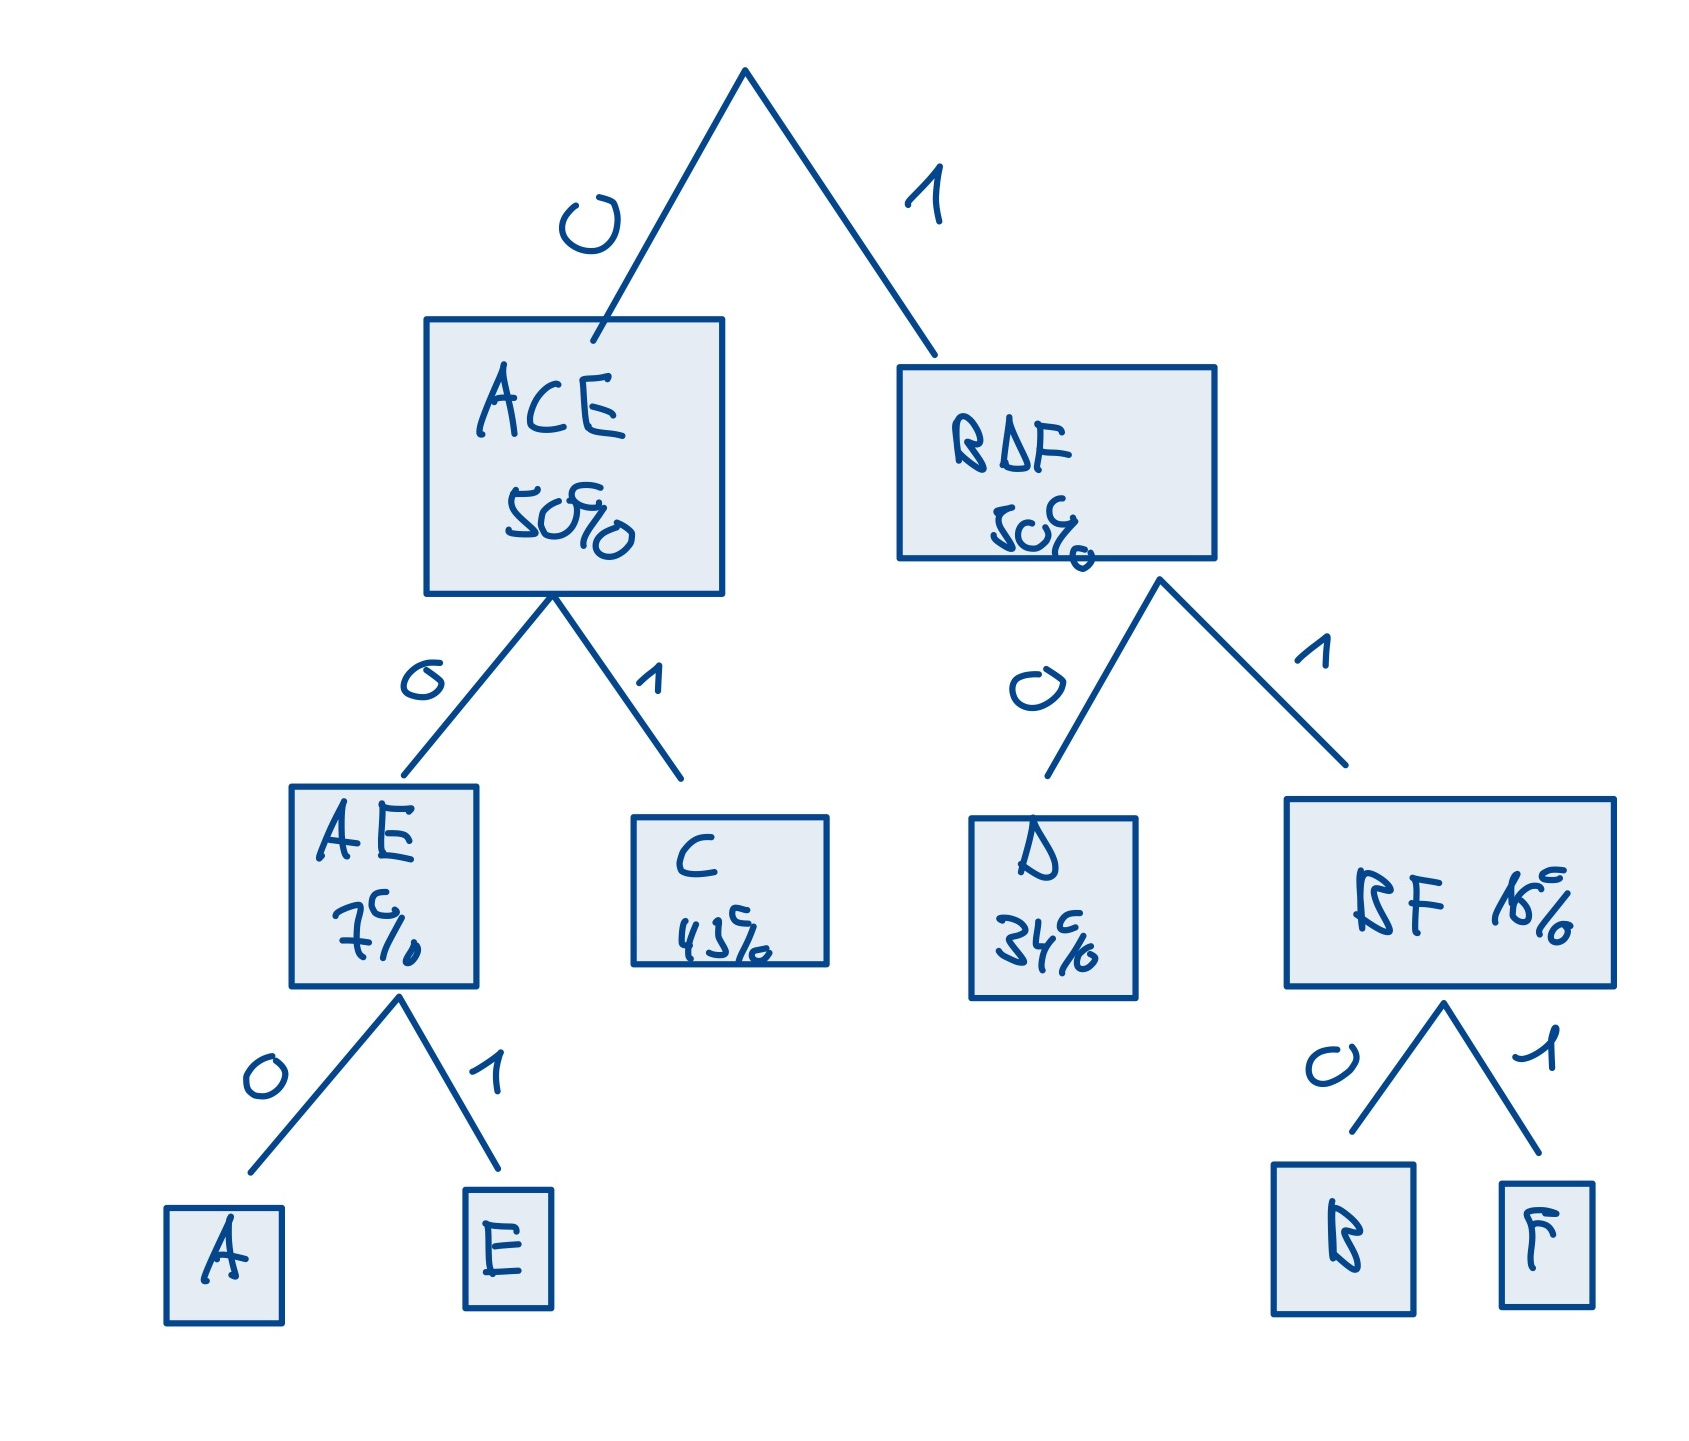
\includegraphics[width = 0.5\textwidth]{GrundlagenInfo/ExamQuestions/Figures/lsg2-2024-1.jpg}
                \end{center}
                \centering
                \begin{tabular}{|c|c|c|}
                \hline
                    Buchstabe & Häufigkeit &  Kodierung  \\ \hline\hline
                   A & 4\% & 000\\ \hline
                   B& 12\% & 110\\  \hline
                   C & 43\% & 01\\  \hline
                   D & 34\% & 10\\  \hline
                   E & 3\% &001 \\  \hline
                   F & 4\% & 111\\  \hline
                \end{tabular}
                    
            \end{solutionorgrid}
            \part[3]
        Um wie viel Prozent verringert sich der Speicherplatzbedarf, wenn man anstatt der ASCII-Kodierung Ihre Kodierung aus Aufgabe (a) verwendet?
        \begin{solutionorgrid}[\stretch{1}]
            Speicherbedarf für 100 Zeichen mit ASCII: $100\cdot 8 = 800$ Bits.

            Speicherbedarf für 100 Zeichen mit der Kodierung aus a.: 
            $$4\cdot 3 + 12\cdot 3 + 43\cdot 2 + 34\cdot 2 + 3\cdot 3 + 4\cdot 3 = 223 \text{ Bits}$$

            Ersparnis: $\frac{800-223}{800} = 0.72125 = 72.125\%$

                
        \end{solutionorgrid}

        \end{parts}
       

        
        \clearpage
        \question[3]
        Ein Text besteht aus den folgenden Buchstaben mit den angegebenen relativen Häufigkeiten. Nutzen Sie den \textbf{Algorithmus von Huffman,} um eine binäre Kodierung für die Buchstaben zu finden. Geben Sie den Lösungsweg an und tragen Sie die gefundene Kodierung in die Tabelle ein.
        \begin{table}[h!]
            \centering
            \begin{tabular}{|c|c|c|}
            \hline
                Buchstabe & Häufigkeit &  Kodierung \hspace{3cm} \\ \hline\hline
               A & 3\% & \\[10pt] \hline
               B& 15\% & \\[10pt]  \hline
               C & 59\% & \\[10pt]  \hline
               D & 10\% & \\[10pt]  \hline
               E & 4\% & \\[10pt]  \hline
               F & 9\% & \\[10pt]  \hline
            \end{tabular}
        \end{table}
        \begin{solutionorgrid}[\stretch{1}]
            \begin{center}
                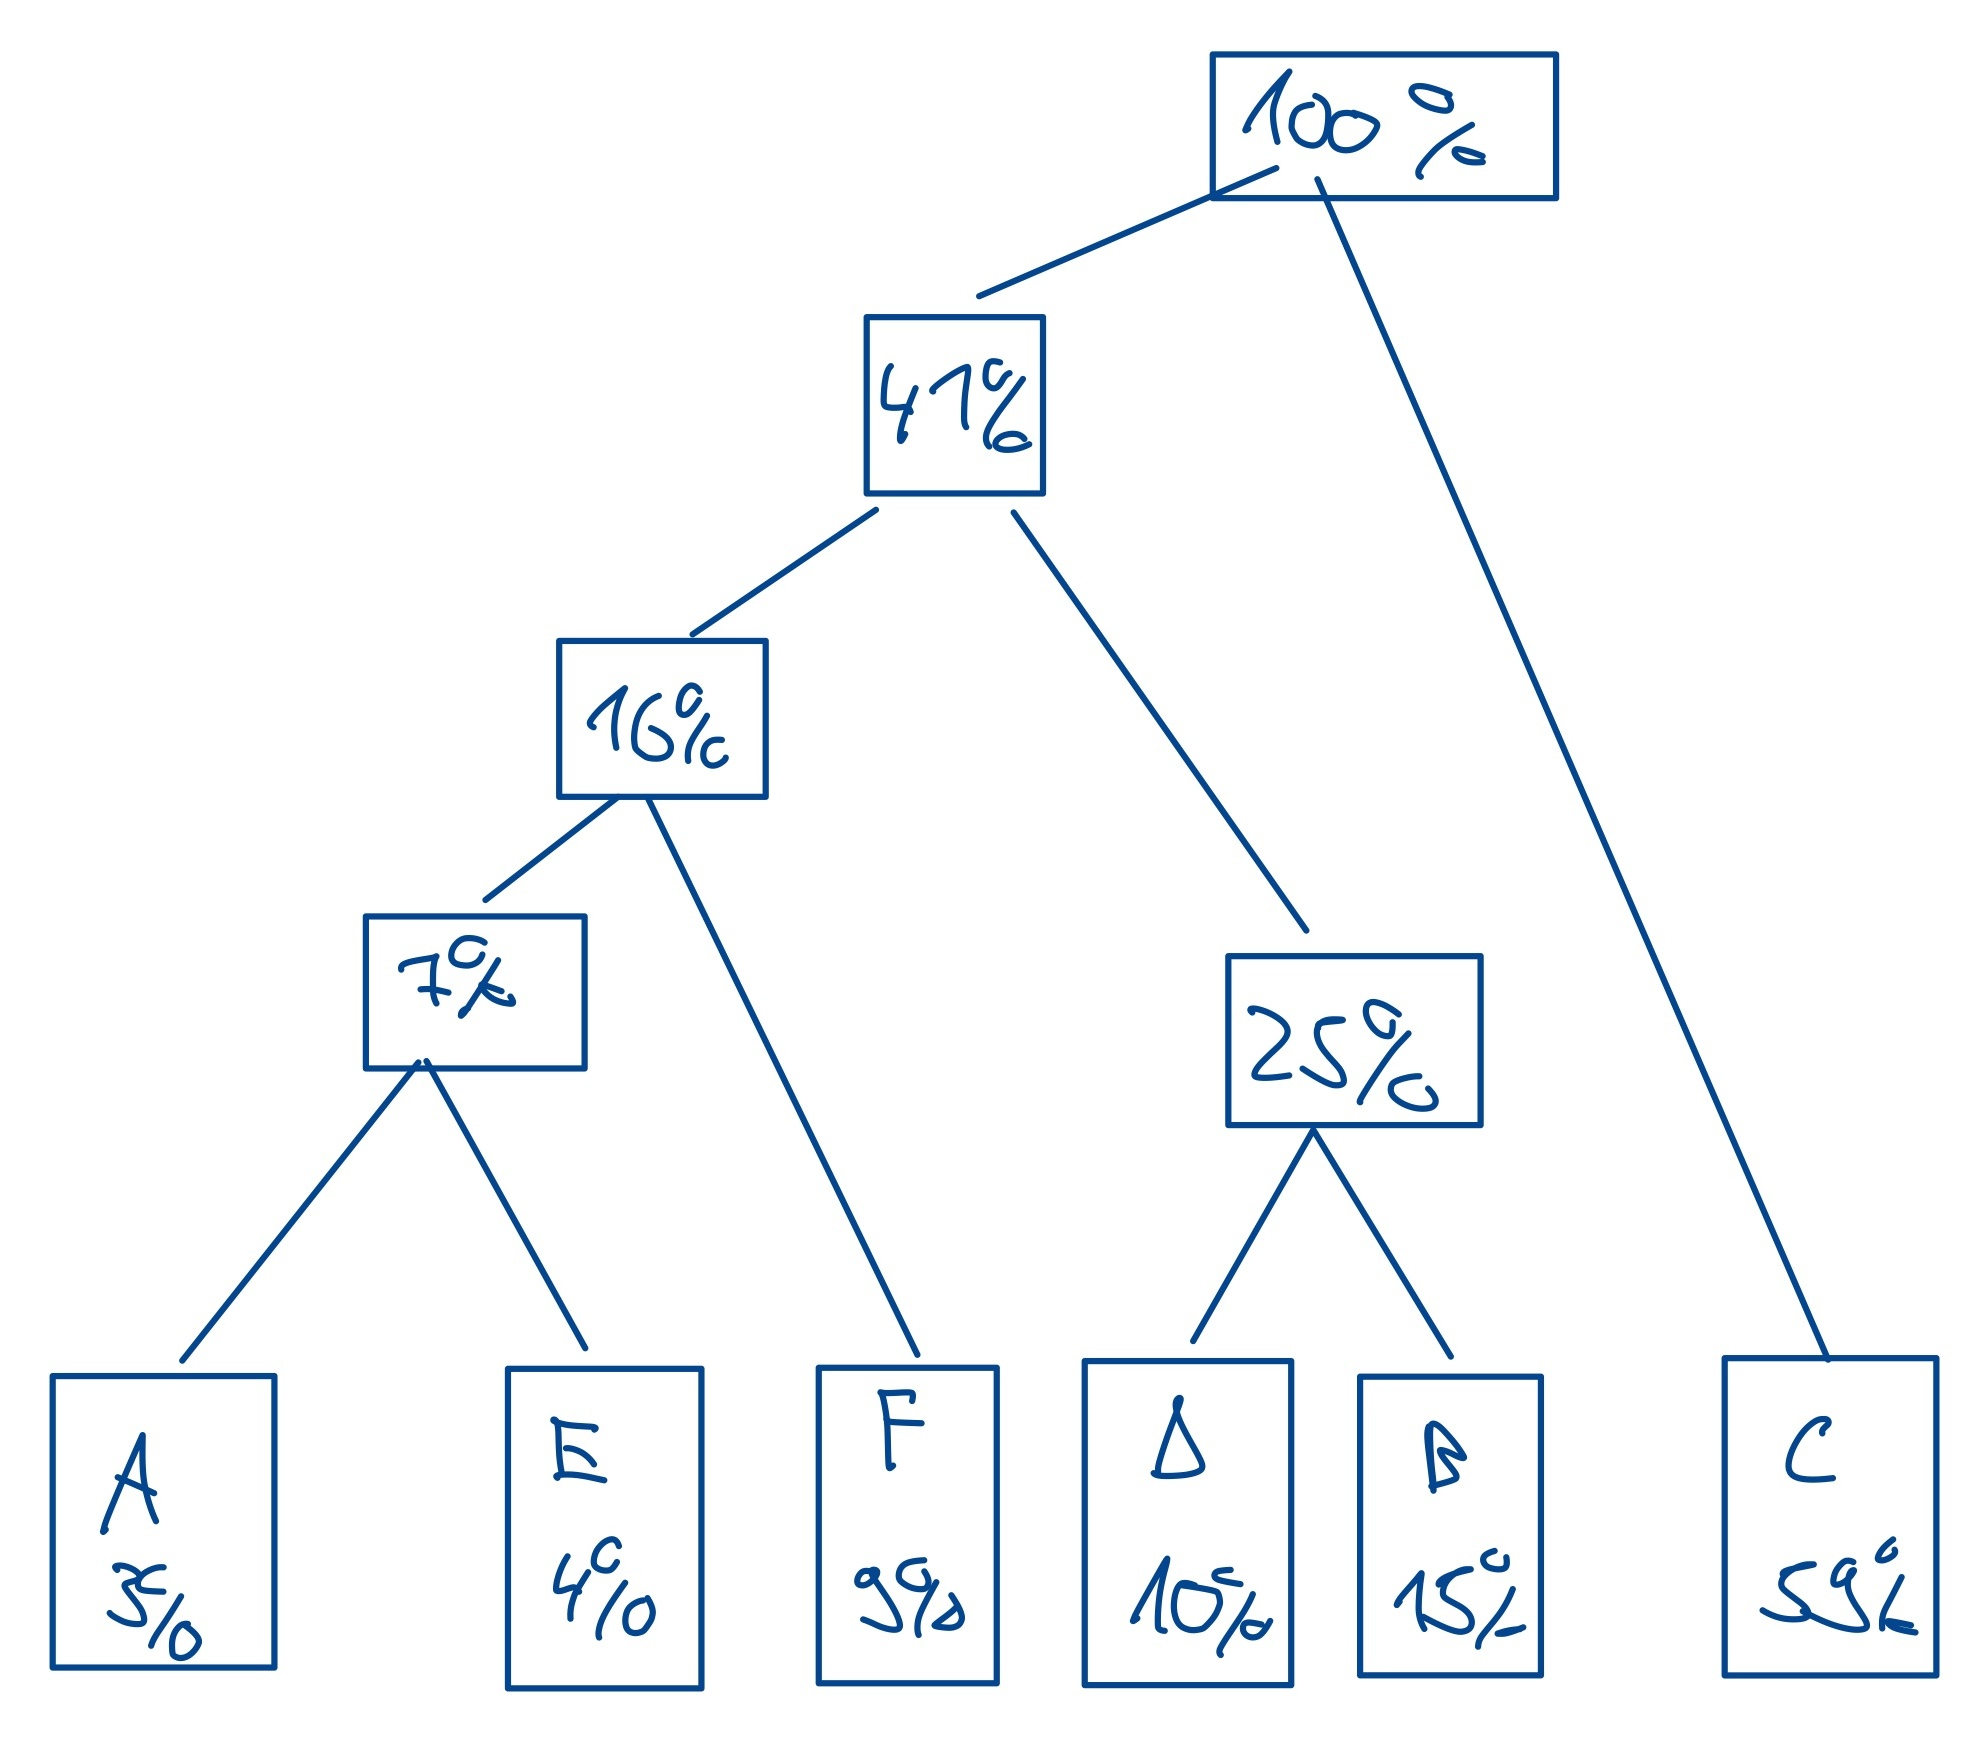
\includegraphics[width = 0.5\textwidth]{GrundlagenInfo/ExamQuestions/Figures/lsg3-2024-3.jpg}
            \end{center}
            \centering
            \begin{tabular}{|c|c|c|}
            \hline
                Buchstabe & Häufigkeit &  Kodierung  \\ \hline\hline
               A & 3\% & 0000\\ \hline
               B& 15\% & 011\\  \hline
               C & 59\% & 1\\  \hline
               D & 10\% & 010\\  \hline
               E & 4\% & 0001\\  \hline
               F & 9\% & 001\\  \hline
            \end{tabular}
        \end{solutionorgrid}
        \clearpage
        \question[3]
        Betrachten Sie die folgenden Wahrscheinlichkeitsverteilung der vier Buchstaben
        
        A - 60\%, B - 20\%, C - 10\%, D - 10\%.

        Die arithmetische Kodierung eines Textes ist \emph{0.755, Textlänge 3}. Wie lautet der unkomprimierte Text?
        \smallskip
        \begin{solutionorgrid}[\stretch{1}]
            \begin{center}
                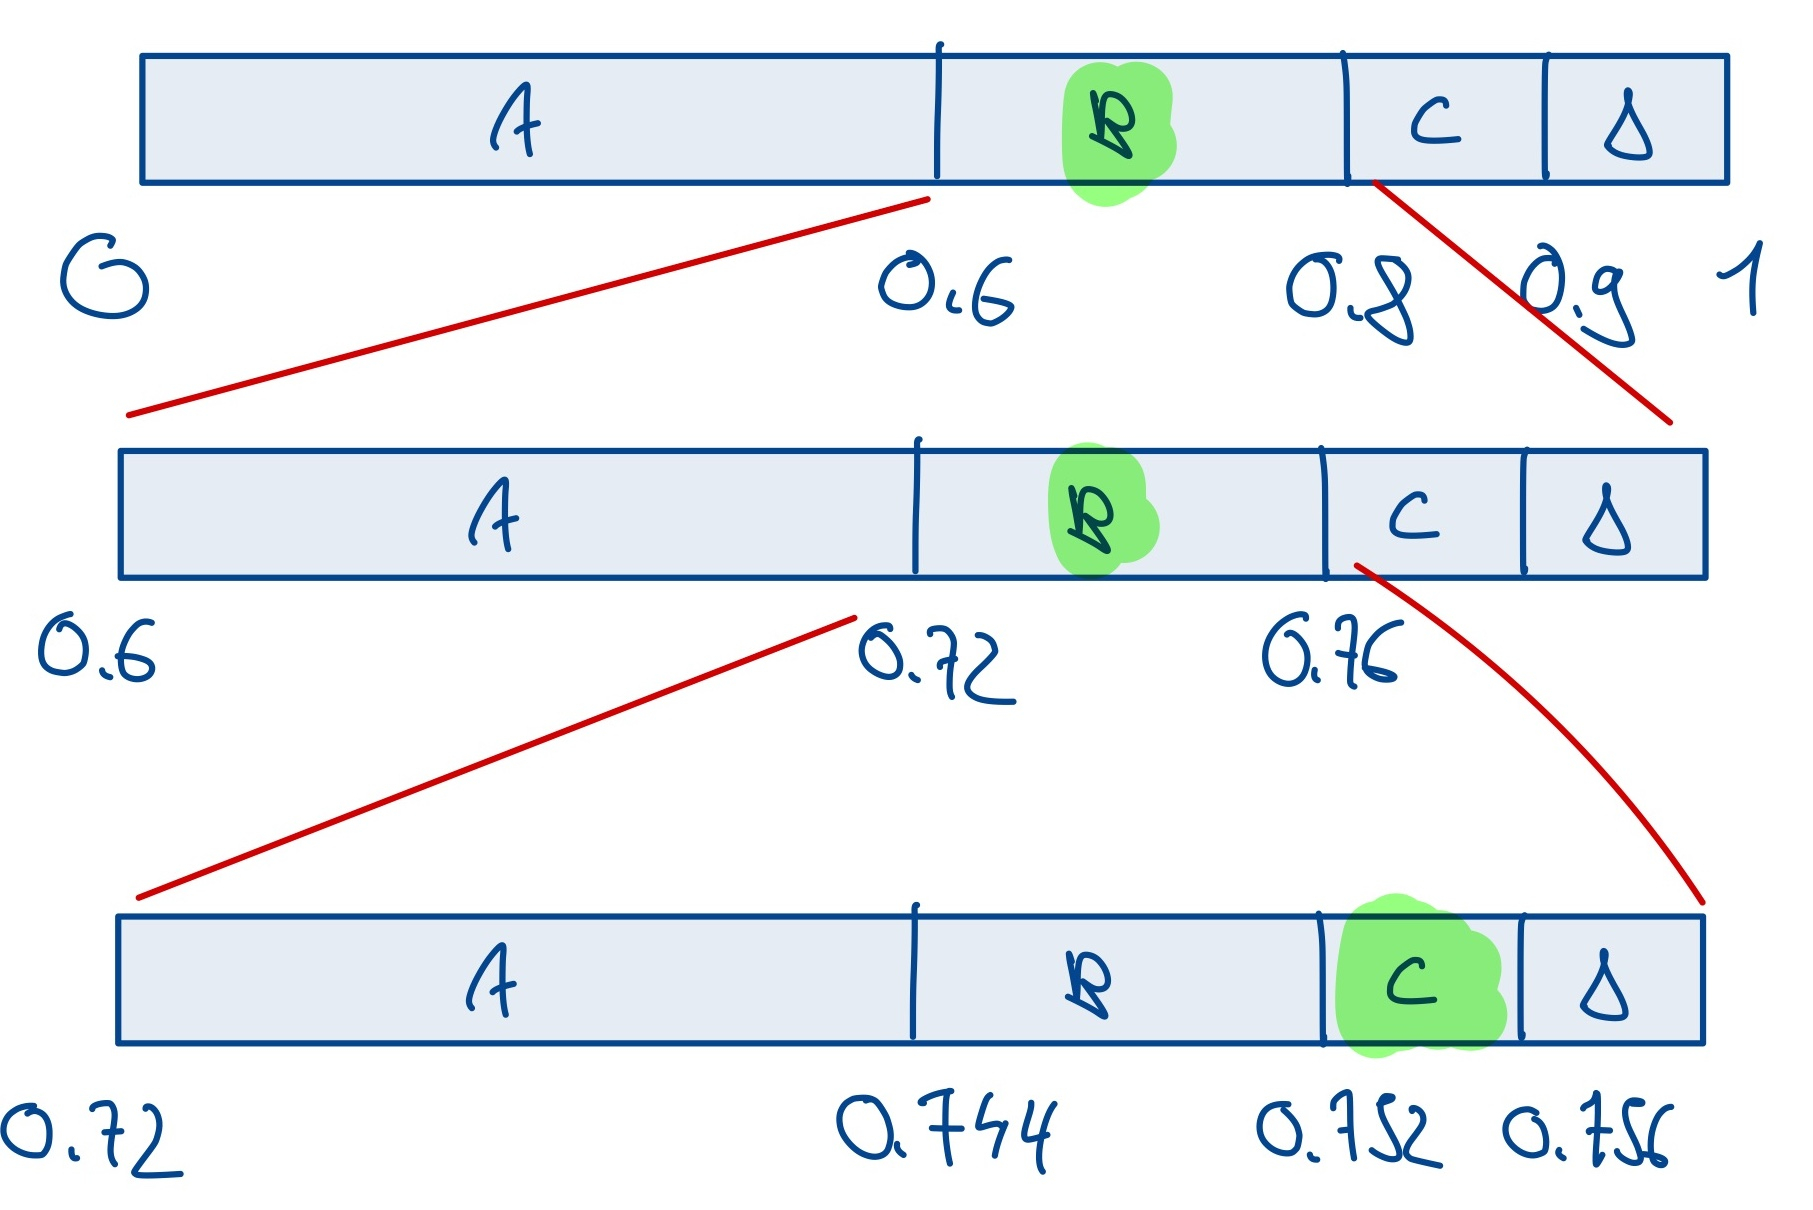
\includegraphics[width = 0.5\textwidth]{GrundlagenInfo/ExamQuestions/Figures/lsg4b-2024-5.jpg}
            \end{center}
            Das kodierte Wort ist BBC.
        \end{solutionorgrid}
        % \begin{parts}
        %     \part[3]
        % Bestimmen Sie die arithmetische Kodierung des Textes DADA als Intervall.
        
        % \begin{solutionorgrid}[\stretch{1}]
        %     \begin{center}
        %         \includegraphics[width = 0.5\textwidth]{lsg4-2024-4.jpg}
        %     \end{center}

        %     Die arithmetische Kodierung von DADA lautet [0.954, 0.9576[
        % \end{solutionorgrid}
        % \part[3]
        % Ein Text wird kodiert mit 0.755 und Textlänge 3. Wie lautet der unkomprimierte Text?
        % \smallskip
        % \begin{solutionorgrid}[\stretch{1}]
        %     \begin{center}
        %         
\includegraphics[width = 0.5\textwidth]{lsg4b-2024-5.jpg}
        %     \end{center}
        %     Das kodierte Wort ist BBC.
        % \end{solutionorgrid}

        % \end{parts}

        \clearpage
        \section{Fehlerkorrigierende Codes}
        \question
        
        Gegeben ist die Kodierung unten für die vier Informationen "ja", "nein", "vielleicht", "keine Antwort". (Die Leerzeichen in der Kodierung dienen nur der besseren Übersicht)

        \begin{table}[h!]
            \centering
            \begin{tabular}{|c|c|}
            \hline
                Information &   Kodierung  \\ \hline\hline
               Ja &  1111 1111\\ \hline
               Nein &  0000 0000\\  \hline
               vielleicht & 1111 1000  \\  \hline
               keine Antwort & 1010 1010  \\  \hline
            \end{tabular}
        \end{table}
        \begin{parts}
            \part[1] Bestimmen Sie den Abstand der Kodierung.
            \begin{solutionorgrid}[\stretch{2}]
                Abstand = 3
            \end{solutionorgrid}
            \part[1] Wie viele Fehler werden durch diese Kodierung erkannt?
            \begin{solutionorgrid}[\stretch{1}]
                2 Fehler werden erkannt
            \end{solutionorgrid}
            \part[1] Wie viele Fehler kann diese Kodierung korrigieren?
            \begin{solutionorgrid}[\stretch{1}]
                1 Fehler wird korrigiert.
            \end{solutionorgrid}
    
    
        \end{parts}
        
        \clearpage
        \question
        Für eine 1-fehlerkorrigierende Kodierung von Nachrichten der Länge 9 Bits wird die "Kartentrick"-Methode mit einer $3\times3$-Tabelle verwendet (bzw. $4\times4$, wenn man die Kontrollbits dazurechnet). Die Kontrollbits (in rot) werden dabei wie folgt in die Tabelle eingetragen: Die ersten drei Bits in der ersten Zeile von links nach rechts. Die zweiten drei Bits in der letzten Spalte von oben nach unten. Das letzte Kontrollbit wird in die Ecke oben rechts der Tabelle eingetragen.

        Die folgenden Nachrichten werden empfangen. Finden Sie die ursprüngliche Nachricht (samt Kontrollbits), wenn Sie annehmen, dass höchstens 1 Bit umgeflippt wurde.
        \begin{parts}
            \part[1] 100 010 100 \textcolor{red}{011 011 0}
            \begin{solutionorgrid}[\stretch{1}]

                \centering
            \begin{tabular}{|c|c|c||c|}
            \hline
                 0&1&1&0     \\ \hline\hline
                 1&0&\textbf{0}&0     \\ \hline
                 0&1&0&1     \\ \hline
                 1&0&0&1    \\ \hline
            \end{tabular}

            Die ursprüngliche Nachricht lautet : 101 010 100 011 011 0

                
            \end{solutionorgrid}
            \part[1] 110 001 100 \textcolor{red}{011 011 0}
            \begin{solutionorgrid}[\stretch{1}]

                  \centering
            \begin{tabular}{|c|c|c||c|}
            \hline
                 0&1&1&0     \\ \hline\hline
                 1&1&0&0     \\ \hline
                 0&0&1&1     \\ \hline
                 1&0&0&1    \\ \hline
            \end{tabular}
            
            Die Nachricht enthält keinen Fehler (oder mehr als einer)

            \end{solutionorgrid}
        
            \part[1] 001 101 111 \textcolor{red}{010 101 0}
            \begin{solutionorgrid}[\stretch{1}]

                \centering
                \begin{tabular}{|c|c|c||c|}
                \hline
                     0&1&\textbf{0}&0     \\ \hline\hline
                     0&0&1&1     \\ \hline
                     1&0&1&0     \\ \hline
                     1&1&1&1    \\ \hline
                \end{tabular}
                
                Die ursprüngliche Nachricht lautet : 001 101 111 011 101 0
                
            \end{solutionorgrid}
        \end{parts}

        \clearpage
        \question[3]
        Zeichnen Sie einen 4 dimensionalen Hyperwürfel. Nehmen Sie 0001 und 1010 als gültige Code-Wörter und ergänzen Sie die Kodierung mit möglichst vielen weiteren Code-Wörtern, sodass die Kodierungen 1-fehler\emph{erkennend} ist.
        \begin{solutionorgrid}[\stretch{1}]
            Mehrere Lösungen mit fünf gültigen Wörter möglich. z.B.

                \begin{center}
                    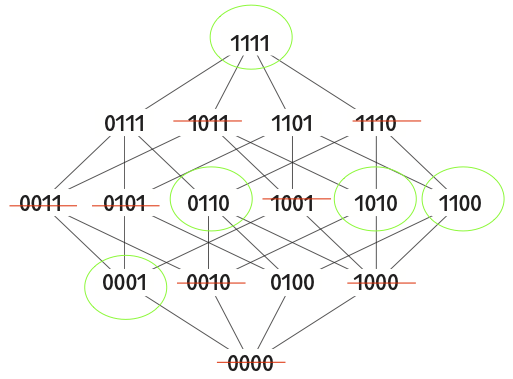
\includegraphics[width = 0.5\textwidth]{GrundlagenInfo/ExamQuestions/Figures/hyperWuerfelEx24.png}
                \end{center}

                Codewörter: 0001, 1010, 0110, 1100, 1111

                Punkte: 1P Für alle möglichen Codes der Länge 4.

                1P für alle Verbindungen im Hyperwürfel.

                1P Für 5 gültige Codewörter


        \end{solutionorgrid}
        
        
        

       
    

        \clearpage
        \fillwithgrid{\stretch{1}}

\end{questions}
